\documentclass{skyalert-report}

%% ══════════════════════════════════════════════════════════════════════════
%%  DATOS DE LA INSTALACIÓN — Cyti-Uagro
%% ══════════════════════════════════════════════════════════════════════════

\sitename{Cyti-Uagro}
\sitelocation{Acapulco, Gro.}
\siteaddress{De las Colinas 37, Las Playas, 39390 Acapulco de Ju\'arez, Gro.}
\sitemaps{https://maps.app.goo.gl/MRohLhQKoLeVw6FEA}
\sitelat{16.835021\textdegree{} N}
\sitelong{99.898257\textdegree{} W}
\sitealt{11.0 msnm}
\seismiczone{Tipo D}

\stationid{AISensor003}
\sensormodel{AS-Explorer Board E-C111G}
\installdate{27/03/2026}
\folio{Ruta-Guerero-01-2026}
\reportid{2026-Gro-001}

\authorname{Isaac P\'erez}
\supportnames{Jorge Giles \& Omar Barrag\'an}
\coverlogo{1}

%% ── Contactos en sitio ────────────────────────────────────────────────────
\newcommand{\contactoA}{M. C. Leopoldo Rodriguez\newline{\small Director Cyti-Uagro}\newline{\small +52 1 744 136 6063}}
\newcommand{\contactoB}{Ing. Ernesto Torrez\newline{\small Jefe de Redes Computacionales}\newline{\small +52 1 55 1954 3344}}

%% ══════════════════════════════════════════════════════════════════════════
\begin{document}

%% ===== PÁG 1: PORTADA =====================================================
\makecover

%% ===== PÁG 2: DATOS GENERALES =============================================
\setheadertext{Datos Generales}
\setfootertext{AISensor003 \textperiodcentered{} Acapulco, Gro. \textperiodcentered{} 27/03/2026}

\sectionhead{Datos Generales de la Instalaci\'on}

\begin{card}
\begin{tabular}{@{}p{0.46\textwidth}p{0.46\textwidth}@{}}
\datafield{Nombre del Sitio}{Cyti-Uagro}&
\datafield{Fecha de Instalaci\'on}{27/03/2026}\\
\datafield{Folio / ID de Reporte}{2026-Gro-001}&
\datafield{Zona S\'ismica}{Tipo D}\\
\end{tabular}%

\begin{tabular}{@{}p{0.95\textwidth}@{}}
\datafield{Direcci\'on}{De las Colinas 37, Las Playas, 39390 Acapulco de Ju\'arez, Gro.}\\
\datafield{Google Maps}{\url{https://maps.app.goo.gl/MRohLhQKoLeVw6FEA}}\\
\end{tabular}%

\begin{tabular}{@{}p{0.30\textwidth}p{0.30\textwidth}p{0.30\textwidth}@{}}
\datafield{Latitud}{16.835021\textdegree{} N}&
\datafield{Longitud}{99.898257\textdegree{} W}&
\datafield{Altitud}{11.0 msnm}\\
\end{tabular}%

\begin{tabular}{@{}p{0.46\textwidth}p{0.46\textwidth}@{}}
\datafield{Contacto en Sitio (1)}{\contactoA}&
\datafield{Contacto en Sitio (2)}{\contactoB}\\
\end{tabular}%
\end{card}

\sectionhead{Detalles de la Estaci\'on S\'ismica}

\begin{tcolorbox}[
  enhanced,colback=tablebg,colframe=divider,boxrule=0.4pt,
  arc=4pt,left=0pt,right=0pt,top=0pt,bottom=0pt,
  shadow={0.4mm}{-0.4mm}{0mm}{black!8}
]
{\footnotesize\setlength{\tabcolsep}{3pt}\raggedright
\begin{tabular}{@{\hspace{4pt}}
  >{\bfseries\raggedright\arraybackslash}p{0.20\textwidth}
  >{\raggedright\arraybackslash}p{0.15\textwidth}
  >{\raggedright\arraybackslash}p{0.08\textwidth}
  >{\raggedright\arraybackslash}p{0.17\textwidth}
  >{\raggedright\arraybackslash}p{0.11\textwidth}
  >{\raggedright\arraybackslash}p{0.12\textwidth}@{\hspace{4pt}}}
\rowcolor{darkbg}
\thead{Dispositivo}&
\thead{Modelo}&
\thead{ID/SN}&
\thead{Ubicaci\'on}&
\thead{Propiedad}&
\thead{Estado}\\
\rowcolor{white}
GPU NVIDIA & Jetson Orin Nano & 003 & Site de redes & SkyAlert & \chipok{Activo}\\
\rowcolor{tablerow}
Sensor S\'ismico principal & ASExplorer E-C111G & 0730B201 & Site de redes & SkyAlert & \chipok{Activo}\\
\rowcolor{white}
Sensor S\'ismico secundario & SKYACC & 003 & Site de redes & SkyAlert & \chipok{Activo}\\
\rowcolor{tablerow}
M\'odem / Router & Ninguno & -- & N/A & -- & \chipna{N/A}\\
\rowcolor{white}
Antena Alta Ganancia & Ninguno & -- & N/A & -- & \chipna{N/A}\\
\rowcolor{tablerow}
Regulador de Voltaje & Koblenz &  & Site de redes & SkyAlert & \chipok{Activo}\\
\rowcolor{white}
Bocina / Altavoz & Ninguna & -- & N/A & -- & \chipna{N/A}\\
\rowcolor{tablerow}
UPS / Bater\'ia & Ninguna & -- & N/A & -- & \chipna{N/A}\\
\end{tabular}}
\end{tcolorbox}

\vspace{5mm}
\noindent
\begin{minipage}[t]{0.24\textwidth}\kpiblock{\faIcon{microchip}}{5}{Dispositivos Activos}\end{minipage}\hfill
\begin{minipage}[t]{0.24\textwidth}\kpiblock{\faIcon{wifi}}{Fibra \'optica}{Conectividad}\end{minipage}\hfill
\begin{minipage}[t]{0.24\textwidth}\kpiblock{\faIcon{shield-alt}}{24 bit}{Resoluci\'on ADC}\end{minipage}\hfill
\begin{minipage}[t]{0.24\textwidth}\kpiblock{\faIcon{clock}}{< 0.1s}{Latencia}\end{minipage}

\newpage

%% ===== PÁG 3: EVIDENCIA FOTOGRÁFICA =======================================
\setheadertext{Evidencia Fotogr\'afica}

\sectionhead{Evidencia Fotogr\'afica de la Instalaci\'on}

\subsectionlabel{Ubicaci\'on del Sitio}

\noindent
\begin{minipage}[t]{0.32\textwidth}
\photoframe{2}{Fachada del Plantel Cyti Uagro}
\end{minipage}\hfill
\begin{minipage}[t]{0.32\textwidth}
\photoframe{3}{Interior del plantel Cyti Uagro}
\end{minipage}\hfill
\begin{minipage}[t]{0.32\textwidth}
\photoframe{4}{Lugar de instalaci\`on (Centro de Computo)}
\end{minipage}

\vspace{4mm}
\subsectionlabel{Instalaci\'on de la Estaci\'on}

\noindent
\begin{minipage}[t]{0.32\textwidth}
\photoframe{5}{Jetson y Arduino instalado}
\end{minipage}\hfill
\begin{minipage}[t]{0.32\textwidth}
\photoframe{6}{Sensor s\'ismico principal}
\end{minipage}\hfill
\begin{minipage}[t]{0.32\textwidth}
\photoframe{7}{Sensor s\'ismico secundario}
\end{minipage}

\vspace{3mm}\noindent
\begin{minipage}[t]{0.32\textwidth}
\photoframe{8}{Momento de instalaci\`on}
\end{minipage}\hfill
\begin{minipage}[t]{0.32\textwidth}
\photoframe{9}{Momento de instalaci\`on}
\end{minipage}\hfill
\begin{minipage}[t]{0.32\textwidth}
\photoframe{10}{Pruebas de ruido s\`ismico en sitio}
\end{minipage}

\vspace{3mm}
\sectionhead{Apoyo en Instalaci\'on}

\begin{card}
\begin{tabular}{@{}p{0.30\textwidth}p{0.30\textwidth}p{0.30\textwidth}@{}}
\datafield{Nombre}{Jorge Giles}&
\datafield{Cargo}{Gerente de Operaciones}&
\datafield{Fecha}{27/03/2026}\\
\datafield{Nombre}{Omar Barrag\'an}&
\datafield{Cargo}{Desarrollador Full Stack}&
\datafield{Fecha}{27/03/2026}\\
\end{tabular}%
\end{card}

\newpage

%% ===== PÁG 4: VALIDACIÓN DE SEÑAL =========================================
\setheadertext{Validaci\'on de Se\~nal}

\sectionhead{Validaci\'on de Se\~nal S\'ismica en Tiempo Real}

\begin{tcolorbox}[
  enhanced,colback=tablebg,colframe=divider,boxrule=0.4pt,
  arc=4pt,left=0pt,right=0pt,top=0pt,bottom=0pt,
  shadow={0.4mm}{-0.4mm}{0mm}{black!8}
]
{\small\setlength{\tabcolsep}{4pt}
\begin{tabular}{@{\hspace{4pt}}
  >{\bfseries\raggedright\arraybackslash}p{0.42\textwidth}
  >{\raggedright\arraybackslash}p{0.28\textwidth}
  >{\raggedright\arraybackslash}p{0.16\textwidth}@{\hspace{4pt}}}
\rowcolor{darkbg}
\thead{Par\'ametro}&
\thead{Valor}&
\thead{Estado}\\
\rowcolor{white}
Nivel de ruido s\'ismico (RMS)&%
\begin{tikzpicture}[baseline=1.5pt]
  \fill[divider,rounded corners=1pt](0,0)rectangle(2.2cm,5pt);
  \fill[greenaccent,rounded corners=1pt](0,0)rectangle(0.66cm,5pt);
\end{tikzpicture}&\chipok{Aceptable}\\
\rowcolor{tablerow}
Frecuencia de muestreo&100 sps&\chipok{OK}\\
\rowcolor{white}
Latencia de transmisi\'on&< 0.1 s&\chipok{OK}\\
\rowcolor{tablerow}
Uptime de conexi\'on&99.8\%&\chipok{OK}\\
\rowcolor{white}
SNR (Signal-to-Noise Ratio)&--&\chipwarn{Pendiente}\\
\rowcolor{tablerow}
Resoluci\'on del ADC&24 bits&\chipok{OK}\\
\rowcolor{white}
Drift de reloj (GPS sync)&< 1 ms&\chipok{OK}\\
\end{tabular}}
\end{tcolorbox}

\vspace{5mm}
\subsectionlabel{Medici\'on de Ruido S\'ismico en Sitio}

\begin{center}
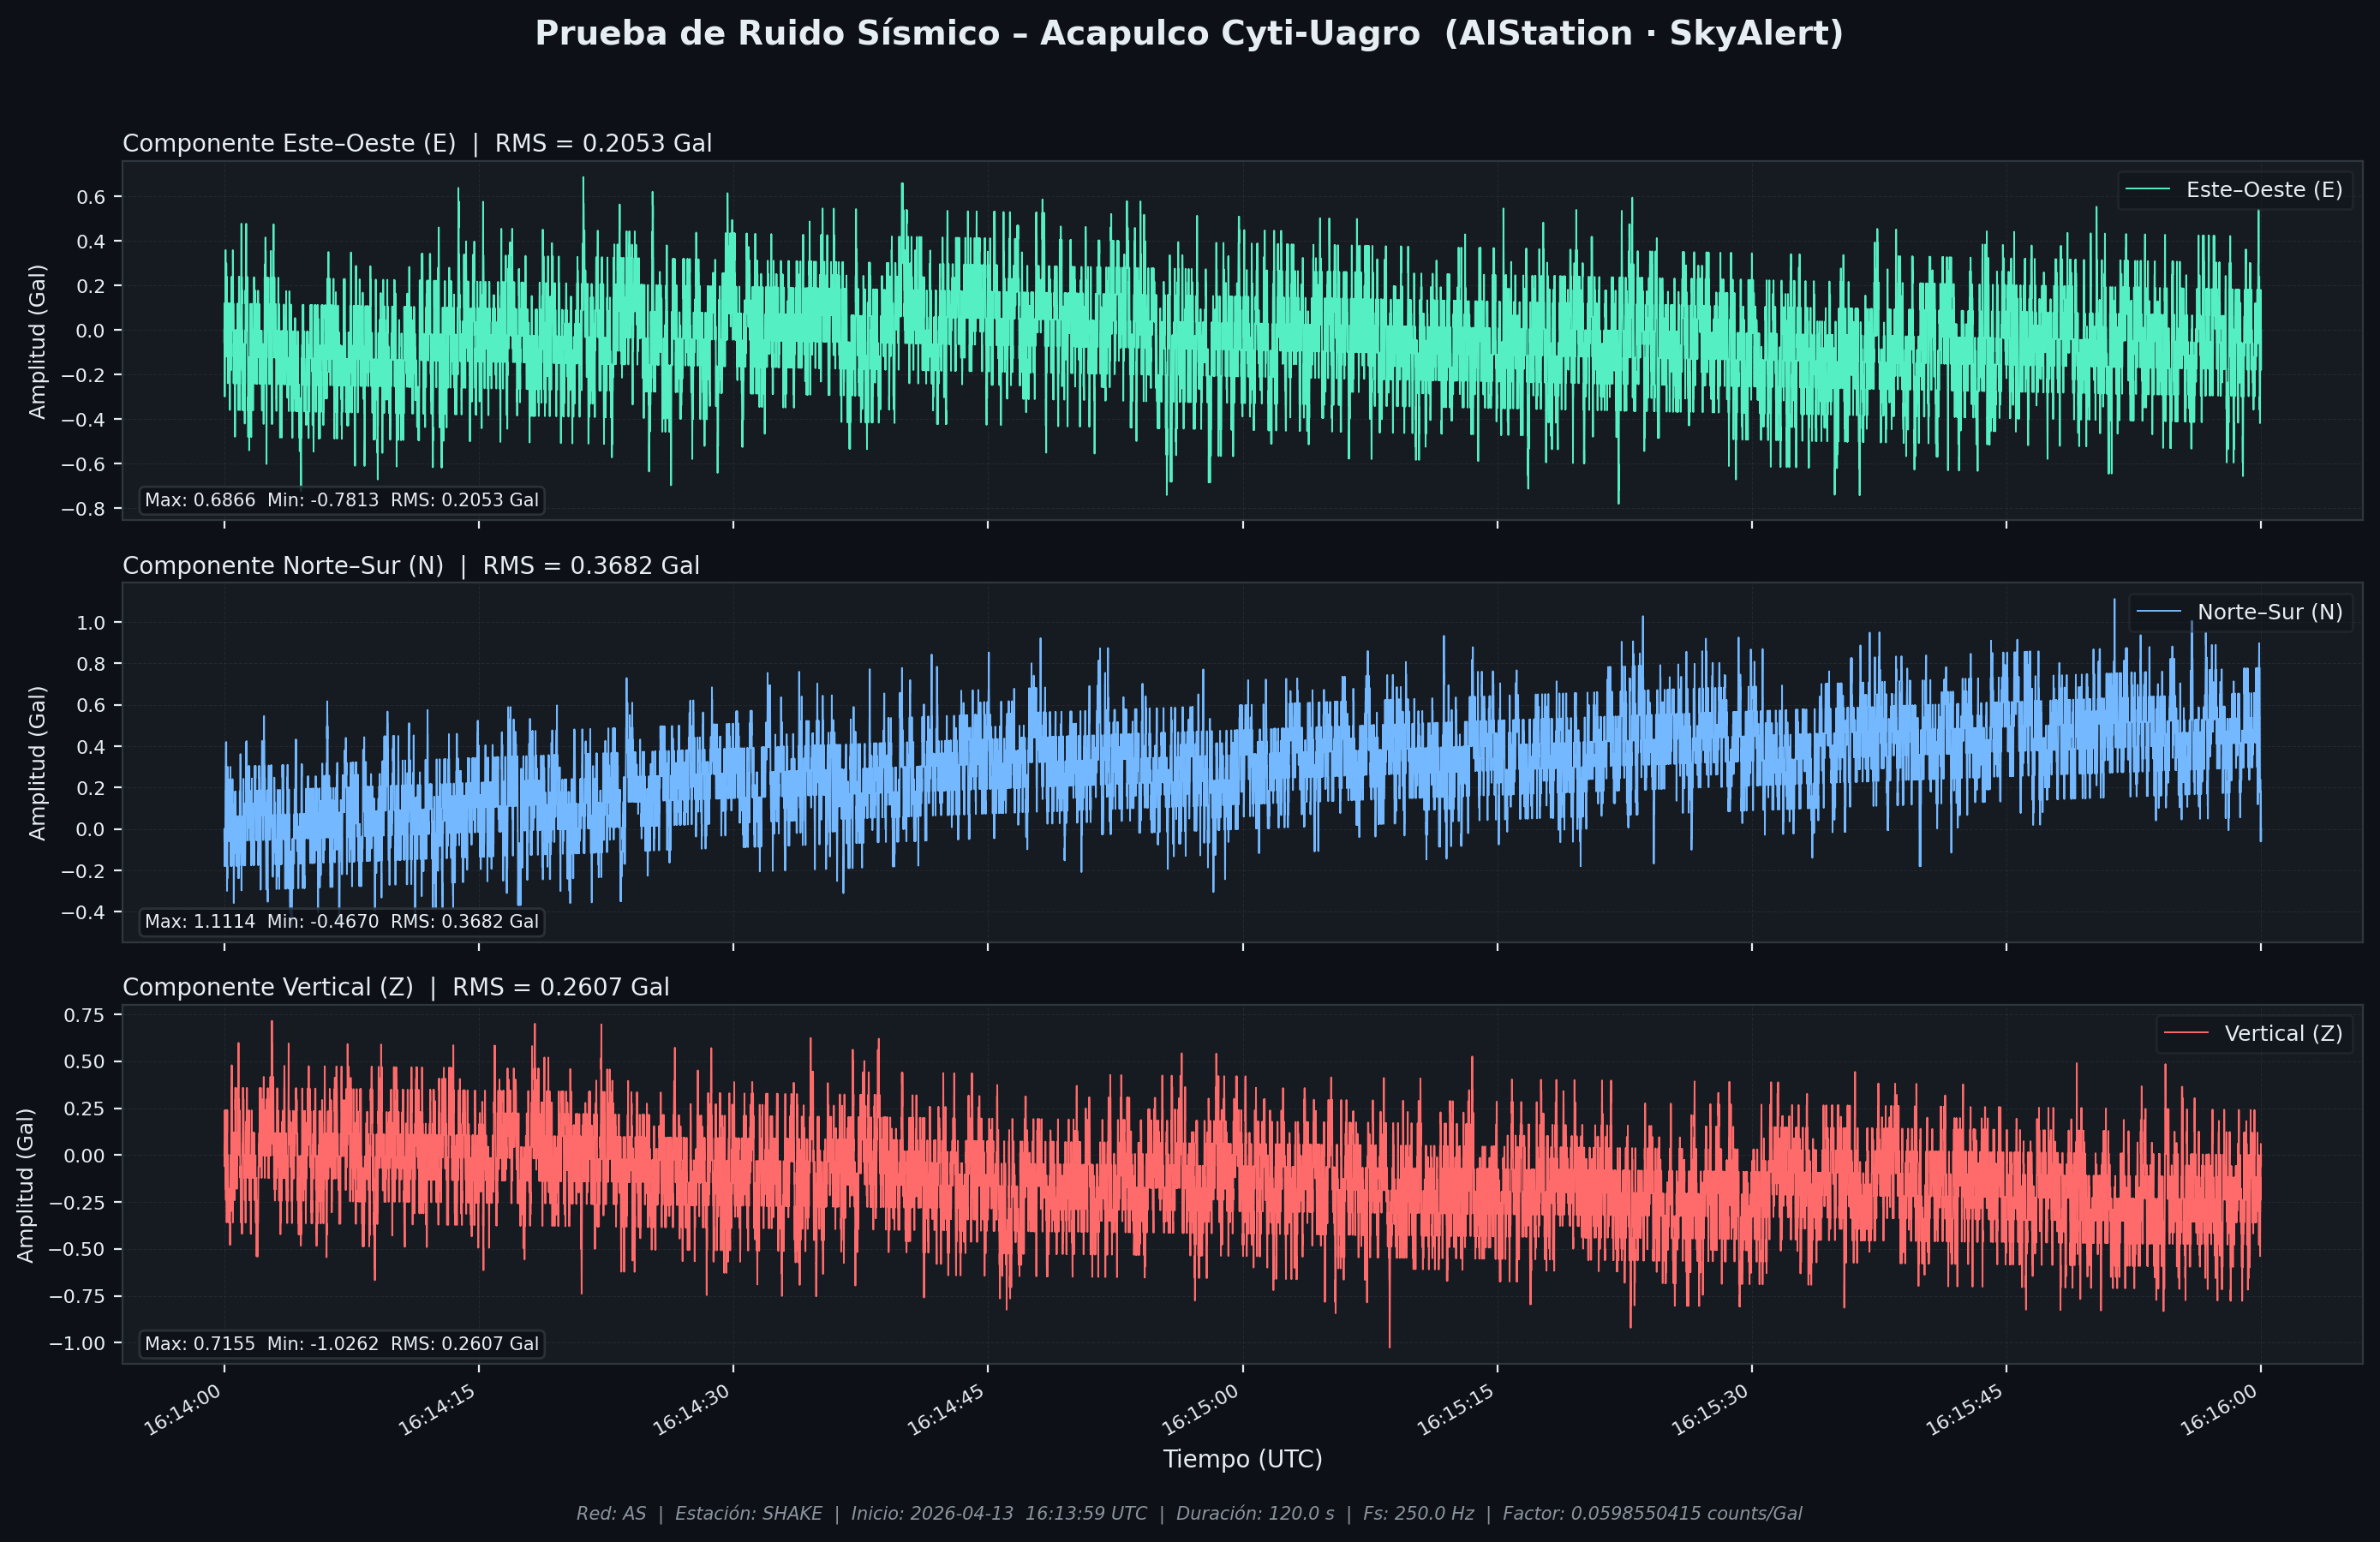
\includegraphics[width=\textwidth]{11}\\[2mm]
{\small\itshape\textcolor{steel}{Formas de onda de aceleraci\'on registradas durante la medici\'on de ruido s\'ismico en sitio.}}
\end{center}

\newpage

%% ===== PÁG 5: PRUEBA MQTT =================================================
\setheadertext{Prueba MQTT}

\sectionhead{Prueba MQTT -- Mensajes de Anomal\'ia a AWS}

\begin{tcolorbox}[
  enhanced,colback=mqttbg,colframe=mqttframe,boxrule=0.5pt,
  arc=4pt,left=8pt,right=8pt,top=6pt,bottom=6pt,
  shadow={0.5mm}{-0.5mm}{0mm}{black!20}
]
{\ttfamily\small\textcolor{mqttgreen}{\faIcon{terminal}\enspace skyalert-mqtt-client}}%
\hfill
\begin{tikzpicture}[baseline=1pt]
  \node[fill=mqttgreen!20!mqttbg,rounded corners=2pt,inner xsep=4pt,inner ysep=1.5pt]{%
    \bfseries\tiny\textcolor{mqttgreen}{\textbullet{} CONNECTED}%
  };
\end{tikzpicture}\\[3mm]
{\ttfamily\footnotesize
\textcolor{mqttcyan}{broker}\hspace{10mm}\textcolor{mqttdim}{xxxxxxxxxx.iot.us-east-1.amazonaws.com}\\
\textcolor{mqttcyan}{topic}\hspace{11.5mm}\textcolor{mqttdim}{skyalert/earthquake/anomalies}\\
\textcolor{mqttcyan}{mensajes}\hspace{6mm}\textcolor{mqttdim}{4 / 4 (100\%)}\hspace{3mm}\textcolor{mqttgreen}{\faIcon{check-circle}\enspace PASS -- Todos los mensajes entregados}\\[3mm]
\textcolor{mqttframe}{\% PAYLOAD ANOMAL\'IA DETECTADA}\\
\textcolor{mqttdim}{\{}\\
\hspace{4mm}\textcolor{mqttcyan}{"station\_id":}\hspace{2mm}\textcolor{mqttcyan!70!white}{"AISensor003"},\\
\hspace{4mm}\textcolor{mqttcyan}{"message":}\hspace{4mm}\textcolor{mqttcyan!70!white}{"ANOMALIA DETECTADA + IA ACTIVADA en 2026-03-27 22:30:30.279 (PGA: 161.3 Gals)"},\\
\hspace{4mm}\textcolor{mqttcyan}{"pga\_gals":}\hspace{3mm}\textcolor{accent}{161.31,}%
\hspace{3mm}\textcolor{mqttcyan}{"anomaly\_active":}\hspace{1mm}\textcolor{amberdark}{true},\\
\hspace{4mm}\textcolor{mqttcyan}{"timestamp":}\hspace{2mm}\textcolor{mqttcyan!70!white}{"2026-03-27T22:30:30.280156+00:00"},\\
\hspace{4mm}\textcolor{mqttcyan}{"location\_name":}\textcolor{mqttcyan!70!white}{"Acapulco, Gro."}\\
\textcolor{mqttdim}{\}}
}
\end{tcolorbox}

\vspace{5mm}
\subsectionlabel{Confirmaci\'on en AWS}

\begin{center}
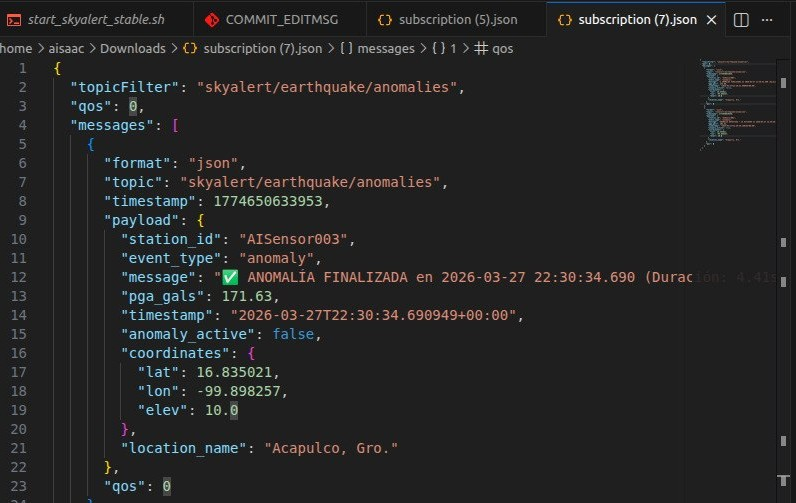
\includegraphics[width=0.5\textwidth]{12}\\[2mm]
{\small\itshape\textcolor{steel}{Confirmaci\'on de recepci\'on de mensajes de anomal\'ia s\'ismica en los servicios AWS.}}
\end{center}

\newpage

%% ===== PÁG 6: OBSERVACIONES Y FIRMAS ======================================
\setheadertext{Observaciones y Aceptaci\'on}

\sectionhead{Comentarios y Observaciones}

\begin{obsbox}
\justifying
Estaci\'on s\'ismica inteligente instalada dentro del site de redes de la Facultad de Ciencias y Tecnolog\'ias de la Informaci\'on de la Cyti Uagro con clima y acceso a fibra \`optica.
\end{obsbox}

\vspace{2mm}
\begin{enumerate}[leftmargin=*,label=\textbf{\textcolor{skyred}{\arabic*.}},itemsep=1pt]
\item La computadora central de la estaci\`on, queda alimentada por la red de intenet local del centro de computo de la Cyti Uagro
\item Sensores s\'ismicos principal y secundario anclados al suelo con cuatro barrenos respectivamente.
\item Se observan condiciones ideales de ruido s\'ismico local para recibir datos de gran calidad.
\item Instalaci\'on de Estaci\'on s\'ismica que cumple los est\'andaresde calidad de SkyAlert 2026.
\end{enumerate}

\vspace{3mm}
\sectionhead{Resumen de Pruebas Realizadas}

\begin{tcolorbox}[
  enhanced,colback=tablebg,colframe=divider,boxrule=0.4pt,
  arc=4pt,left=0pt,right=0pt,top=0pt,bottom=0pt,
  shadow={0.4mm}{-0.4mm}{0mm}{black!8}
]
{\small\setlength{\tabcolsep}{4pt}
\begin{tabular}{@{\hspace{4pt}}
  >{\bfseries\raggedright\arraybackslash}p{0.44\textwidth}
  >{\raggedright\arraybackslash}p{0.14\textwidth}
  >{\raggedright\arraybackslash}p{0.26\textwidth}@{\hspace{4pt}}}
\rowcolor{darkbg}
\thead{Prueba}&
\thead{Resultado}&
\thead{Observaci\'on}\\
\rowcolor{white}
Encendido y arranque del sensor&\chipok{PASS}&Arranque sin errores\\
\rowcolor{tablerow}
Conectividad a internet&\chipok{PASS}&Se\~nal estable\\
\rowcolor{white}
Transmisi\'on de se\~nal s\'ismica&\chipok{PASS}&Latencia < 0.1 s\\
\rowcolor{tablerow}
Barrenado para gabinetes&\chipok{PASS}&Gabinetes fijados\\
\rowcolor{white}
Detecci\'on de anomal\'ia (AI Station)&\chipok{PASS}&IA\_output, Zc, PGA\\
\rowcolor{tablerow}
Env\'io MQTT a AWS IoT Core&\chipok{PASS}&4/4 mensajes (100\%)\\
\rowcolor{white}
Sincronizaci\'on de reloj GPS&\chipok{PASS}&Drift < 10 ms\\
\rowcolor{tablerow}
Est\'andares SkyAlert 2026&\chipok{PASS}&Criterios verificados\\
\end{tabular}}
\end{tcolorbox}

\vspace{4mm}
\sectionhead{Verificaci\'on y Aceptaci\'on}

\noindent
\begin{minipage}[t]{0.48\textwidth}
\signblock{Encargado de la Instalaci\'on}{Ing. Isaac P\'erez}{Especialista en Sismolog\'ia e Instrumentaci\'on Geof\'isica}{27/03/2026}
\end{minipage}\hfill
\begin{minipage}[t]{0.48\textwidth}
\signblock{Encargado del Sitio (Aliado)}{M. C. Leopoldo Rodriguez}{Director Genral de Cyti-Uagro}{27/03/2026}
\end{minipage}

\end{document}
